\documentclass[tikz, border=10pt]{standalone}
\usepackage{tikz}
\usepackage{amsmath, amssymb}
\usetikzlibrary{calc, shapes.geometric, arrows.meta, positioning, fit, backgrounds, shadows}

\newcommand{\fstar}{f^{\ast}}
\newcommand{\metric}{d_{\mathcal{Y}}}
\newcommand{\concat}{\oplus}

% Define styles in preamble (no blank lines allowed inside)
\tikzset{
  % --- Ghost (Background) Styles ---
  ghostnode/.style={
    draw=gray!20, fill=white, text=gray!30, 
    rounded corners=2pt, minimum width=0.9cm, minimum height=0.5cm, font=\scriptsize
  },
  ghostedge/.style={->, draw=gray!20, line width=0.5pt},
  % --- Active (Audit) Styles ---
  activenode/.style={
    draw=black!70, fill=white, text=black!85, drop shadow,
    rounded corners=2pt, minimum width=0.9cm, minimum height=0.5cm, font=\small\bfseries
  },
  referencenode/.style={
    activenode, draw=black!60, dashed, fill=gray!5, text=black!70
  },
  % --- Comparator (The "Test" Diamond) ---
  comparator/.style={
    diamond, aspect=1.3, draw=black!80, fill=white, 
    inner sep=1pt, font=\bfseries\tiny, align=center, drop shadow
  },
  % --- Grouping Boxes ---
  % Increased inner sep to ensure text doesn't touch borders
  groupbox/.style={
    rounded corners=5pt, draw opacity=0.8, fill opacity=0.1, thick, inner sep=6pt
  },
  % --- Text Labels ---
  lawtitle/.style={
    font=\bfseries\small, align=center
  },
  lawdesc/.style={
    font=\scriptsize, align=center, inner sep=2pt, text opacity=0.9
  }
}

\begin{document}

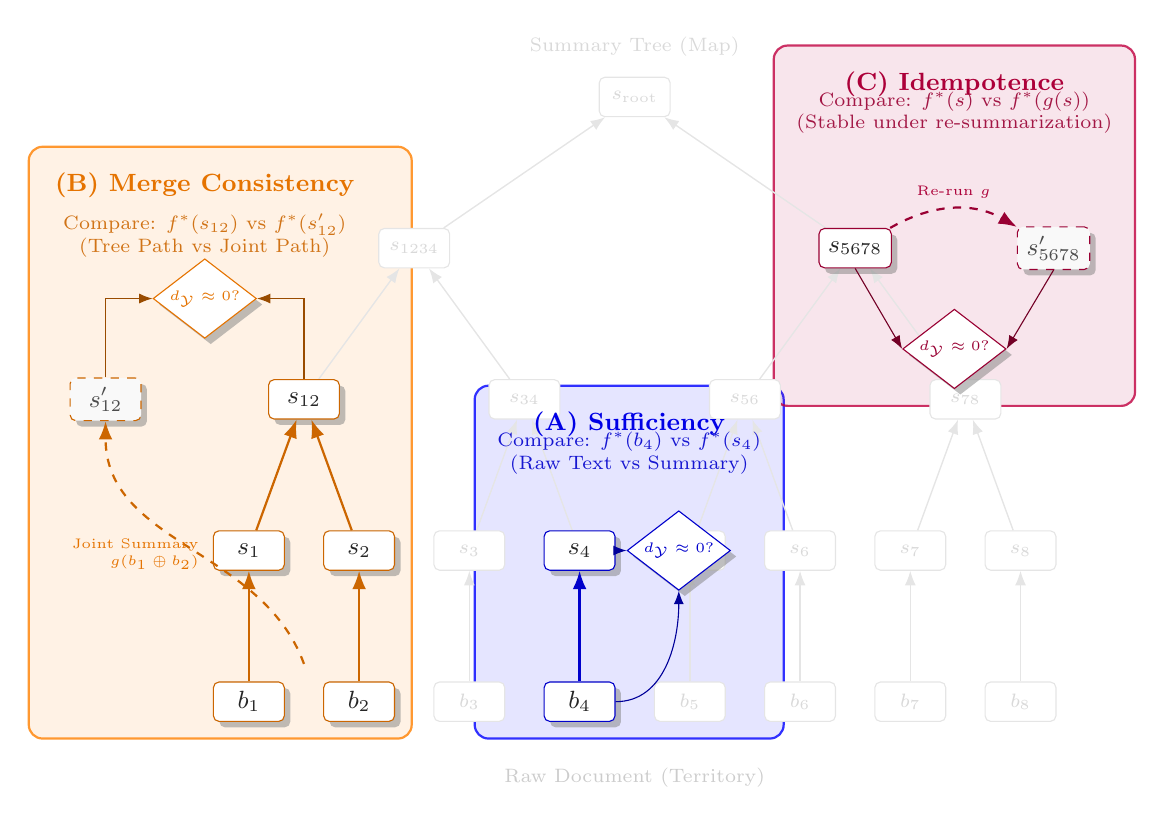
\begin{tikzpicture}[x=1.4cm, y=1.6cm, >=Latex, font=\sffamily]

  % =================================================================================
  % 1. BUILD THE GHOST TREE (Context)
  % =================================================================================
  
  % Level 0: Raw Blocks
  \foreach \i in {1,...,8} {
    \node[ghostnode] (b\i) at (\i, 0) {$b_{\i}$};
  }
  
  % Level 1: Leaf Summaries
  \foreach \i in {1,...,8} {
    \node[ghostnode] (s\i) at (\i, 1.2) {$s_{\i}$};
    \draw[ghostedge] (b\i) -- (s\i);
  }
  
  % Level 2: Merges
  \foreach \i/\j/\k in {1/2/12, 3/4/34, 5/6/56, 7/8/78} {
    \node[ghostnode] (s\k) at ($(\i,1.2)!0.5!(\j,1.2) + (0,1.2)$) {$s_{\k}$};
    \draw[ghostedge] (s\i) -- (s\k);
    \draw[ghostedge] (s\j) -- (s\k);
  }

  % Level 3
  \foreach \i/\j/\k in {12/34/1234, 56/78/5678} {
    \node[ghostnode] (s\k) at ($(s\i)!0.5!(s\j) + (0,1.2)$) {$s_{\k}$};
    \draw[ghostedge] (s\i) -- (s\k);
    \draw[ghostedge] (s\j) -- (s\k);
  }

  % Root
  \node[ghostnode] (root) at ($(s1234)!0.5!(s5678) + (0,1.2)$) {$s_{\text{root}}$};
  \draw[ghostedge] (s1234) -- (root);
  \draw[ghostedge] (s5678) -- (root);

  % Background Labels
  \node[text=gray!40, font=\scriptsize] at (4.5, -0.6) {Raw Document (Territory)};
  \node[text=gray!30, font=\scriptsize] at (4.5, 5.2) {Summary Tree (Map)};


  % =================================================================================
  % 2. SPOTLIGHT A: SUFFICIENCY (Middle)
  % =================================================================================
  
  % Active Nodes
  \node[activenode, draw=blue!80!black] (act_b4) at (b4) {$b_4$};
  \node[activenode, draw=blue!80!black] (act_s4) at (s4) {$s_4$};
  \draw[->, blue!80!black, thick] (act_b4) -- (act_s4);
  
  % Comparator
  \node[comparator, draw=blue!80!black, text=blue!80!black] (comp_A) at ($(act_s4) + (0.9, 0)$) {$d_{\mathcal{Y}} \approx 0?$};
  
  % Comparison Arrows
  \draw[->, blue!60!black] (act_s4.east) -- (comp_A);
  \draw[->, blue!60!black] (act_b4.east) to[out=0, in=-90] (comp_A.south);
  
  % Labels - positioned to maximize space
  \node[lawtitle, text=blue!90!black] (lbl_A) at ($(act_s4)!0.5!(comp_A) + (0, 1.0)$) 
    {(A) Sufficiency};
  \node[lawdesc, text=blue!80!black] (desc_A) at ($(lbl_A.south) + (0, -0.05)$) 
    {Compare: $\fstar(b_4)$ vs $\fstar(s_4)$\\(Raw Text vs Summary)};
    
  % Group Box - Explicitly fitting the description node
  \begin{scope}[on background layer]
    \node[groupbox, draw=blue, fill=blue, fit=(act_b4)(act_s4)(comp_A)(lbl_A)(desc_A)] {};
  \end{scope}


  % =================================================================================
  % 3. SPOTLIGHT B: MERGE CONSISTENCY (Left Side)
  % =================================================================================
  
  % Pipeline Nodes
  \node[activenode, draw=orange!80!black] (act_b1) at (b1) {$b_1$};
  \node[activenode, draw=orange!80!black] (act_b2) at (b2) {$b_2$};
  \node[activenode, draw=orange!80!black] (act_s1) at (s1) {$s_1$};
  \node[activenode, draw=orange!80!black] (act_s2) at (s2) {$s_2$};
  \node[activenode, draw=orange!80!black] (act_s12) at (s12) {$s_{12}$};
  
  % Pipeline Edges
  \draw[->, orange!80!black, thick] (act_b1) -- (act_s1);
  \draw[->, orange!80!black, thick] (act_b2) -- (act_s2);
  \draw[->, orange!80!black, thick] (act_s1) -- (act_s12);
  \draw[->, orange!80!black, thick] (act_s2) -- (act_s12);
  
  % Reference Node
  \node[referencenode, draw=orange!80!black] (ref_s12) at ($(act_s12) + (-1.8, 0)$) {$s'_{12}$};
  
  % Joint Edge
  \draw[->, orange!80!black, dashed, thick] ($(act_b1)!0.5!(act_b2) + (0, 0.3)$) 
    to[out=110, in=-90] 
    node[pos=0.45, left, font=\tiny, align=right, text=orange!90!black, inner sep=1pt] {Joint Summary\\$g(b_1 \concat b_2)$} 
    (ref_s12);

  % Comparator
  \node[comparator, draw=orange!90!black, text=orange!90!black] (comp_B) at ($(act_s12)!0.5!(ref_s12) + (0, 0.8)$) {$d_{\mathcal{Y}} \approx 0?$};
  
  % Comparison Arrows
  \draw[->, orange!60!black] (act_s12.north) |- (comp_B.east);
  \draw[->, orange!60!black] (ref_s12.north) |- (comp_B.west);

  % Labels
  \node[lawtitle, text=orange!90!black, anchor=south] (lbl_B) at ($(comp_B.north) + (0, 0.4)$) 
    {(B) Merge Consistency};
  \node[lawdesc, text=orange!80!black, anchor=north] (desc_B) at (lbl_B.south) 
    {Compare: $\fstar(s_{12})$ vs $\fstar(s'_{12})$\\(Tree Path vs Joint Path)};

  % Group Box
  \begin{scope}[on background layer]
    \node[groupbox, draw=orange, fill=orange, fit=(act_b1)(act_b2)(ref_s12)(comp_B)(act_s12)(lbl_B)(desc_B)] {};
  \end{scope}


  % =================================================================================
  % 4. SPOTLIGHT C: IDEMPOTENCE (Right Side - s5678)
  % =================================================================================
  
  % Active Node
  \node[activenode, draw=purple!80!black] (act_s5678) at (s5678) {$s_{5678}$};
  
  % Regeneration Node
  \node[referencenode, draw=purple!80!black] (regen_s5678) at ($(act_s5678) + (1.8, 0)$) {$s'_{5678}$};
  
  % Regeneration Arrow
  \draw[->, purple!80!black, dashed, thick] (act_s5678) to[out=30, in=150] node[above, font=\tiny, text=purple!90!black] {Re-run $g$} (regen_s5678);
  
  % Comparator
  \node[comparator, draw=purple!80!black, text=purple!80!black] (comp_C) at ($(act_s5678)!0.5!(regen_s5678) + (0, -0.8)$) {$d_{\mathcal{Y}} \approx 0?$};
  
  % Comparison Arrows
  \draw[->, purple!60!black] (act_s5678.south) -- (comp_C.west);
  \draw[->, purple!60!black] (regen_s5678.south) -- (comp_C.east);

  % Labels - Centered above the operation
  \node[lawtitle, text=purple!90!black] (lbl_C) at ($(act_s5678)!0.5!(regen_s5678) + (0, 1.3)$) 
    {(C) Idempotence};
  \node[lawdesc, text=purple!80!black] (desc_C) at ($(lbl_C.south) + (0, -0.05)$) 
    {Compare: $\fstar(s)$ vs $\fstar(g(s))$\\ (Stable under re-summarization)};

  % Group Box
  \begin{scope}[on background layer]
    \node[groupbox, draw=purple, fill=purple, fit=(act_s5678)(regen_s5678)(comp_C)(lbl_C)(desc_C)] {};
  \end{scope}

\end{tikzpicture}
\end{document}